\documentclass[a4paper,12pt,french] {article}

\usepackage[TD]{../../Style}

\begin{document}

\titre{ Exercices - Nombres réels }

\section*{Nature des nombres, encadrement décimal}

\begin{exercice}
\
Parmi les nombres suivants, quelle écriture ne désigne pas le même nombre rationnel que les autres?
$$\frac {25} {45},\ \frac 5 9,\ \frac {30} {36},\ \frac 1 3 + \frac 2 9,\ \frac {-10} {-18}$$
 
\end{exercice}
 
\begin{exercice}

Déterminer le plus petit ensemble auquel appartient chacun de ces nombres: 

$$ \frac {21} 4,\ \frac {15} 5,\ \sqrt 5 ,\ \frac {4+5} {5-2},\ 10^{-5}, 1.78,\ \frac {13} {11},\ 3.65,\ 3.656565 \ldots,\ \sqrt 9,\ \frac {\pi^2} {\pi}$$

\end{exercice}

\begin{exercice}
\
Sur une droite graduée, représenter les nombres entiers en rouge, les nombres rationnels non entiers en vert et les nombres irrationnels en bleu:

$$ -2.5,\ \sqrt 2,\ \frac 1 3,\ \frac 4 2,\ - \pi,\ -1.67,\ 10^{-1}$$

\end{exercice}

\begin{exercice}

Compléter les pointillés par le symbole $\in$ ou $\not\in$ qui convient:

\hspace{-5mm} \begin{tabularx}{\textwidth}{>{\centering\arraybackslash}X >{\centering\arraybackslash}X >{\centering\arraybackslash}X >{\centering\arraybackslash}X >{\centering\arraybackslash}X >{\centering\arraybackslash}X}
$-15.4 \ \ldots \ \Q$ & $\frac 1 {\pi} \ \ldots \ \R$ & $- \sqrt 4 \ \ldots \ \Z$ & $\frac 9 {11} \ \ldots \ \D$ & $\frac {12} 6 \ \ldots \ \N$ & $\frac {\pi} 2 \ \ldots \ \Q$ 
\end{tabularx}

\end{exercice}

\begin{exercice} \

\begin{enumerate}

\item Déterminer l'abcisse de chacun des points de cet axe:
\begin{center}
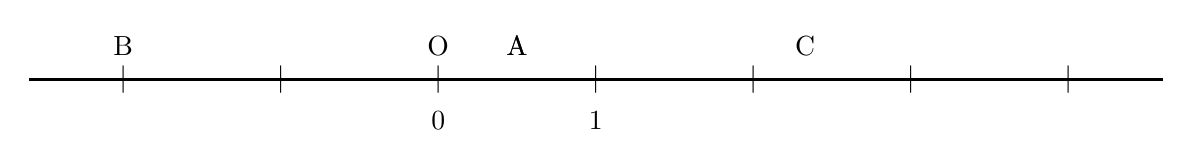
\begin{tikzpicture}
	\draw[thick,-] (-5.2,0) --(9.2,0);
	\foreach \xp in {-4,-2,...,8}{\node[] at (\xp,0) {$\mid$};}
	\node[below=8pt] at (0,0) {0};
    \node[below=8pt] at (2,0) {1};
    \node[] at (1,0) {$\shortmid$};
	\node[above=5pt] at (1,0) {A};
	\node[] at (-4,0) {$\shortmid$};
	\node[above=5pt] at (-4,0) {B};
	\node[] at (4.66,0) {$\shortmid$};
	\node[above=5pt] at (4.66,0) {C};
	\node[] at (0,0) {$\shortmid$};
	\node[above=5pt] at (0,0) {O};
	\node[] at (1,0) {$\shortmid$};
	\node[above=5pt] at (1,0) {A};
	
\end{tikzpicture}
\end{center}
\vspace{3mm}

\item Associer aux réels suivants un point sur la droite des réels ci-dessus:
$$-1,\ \frac 1 4,\ \sqrt 3,\ -\frac 7 2$$

\end{enumerate}
\end{exercice}

\begin{exercice} \

\begin{enumerate}

\item Donner un encadrement décimal d'amplitude $10^{-3}$ de $\sqrt{11}$

\item Donner un encadrement décimal d'amplitude $10^{-4}$ de $\sqrt 2$, puis un arrondi à $10^{-4}$.

\item Donner un encadrement décimal d'amplitude $10^{-2}$ de $1,735$ puis un arrondi à $10^{-2}$.

\end{enumerate}

\end{exercice}

\begin{exercice}
L'une des meilleures et plus simples approximations de $\pi$ est le nombre $\frac {22} 7$. Déterminer la précision de cet arrondi. Même question pour $\frac {333} {106}$.

\textit{ Note: on peut générer une infinité de fractions de plus en plus complexes mais qui approchent de mieux en mieux $\pi$: $\frac {355} {113}, \frac {103993} {33102},  \ldots$. Dans la pratique, on a besoin que d'un arrondi à $10^{-15}$ maximum mais le calcul des décimales de $\pi$ reste un défi intéressant pour tester nos ordinateurs: Aujourd'hui, quelques $62 800$ milliards de décimales ont été calculées ...}
\end{exercice}

\begin{exercice} \textbf {Pour ceux qui sont en avance.} S'inspirer du cours pour retrouver une écriture sous forme de fraction des nombres suivants:
$$0.181818 \ldots ,\ 0.11111 \ldots ,\ 0.9999 \ldots ,\ 0.142857142857 \ldots$$
\end{exercice}

\newpage

\section*{Intervalles, valeur absolue}

\begin{exercice}

Compléter les pointillés par le symbole $\in$ ou $\not\in$ qui convient:

\hspace{-1cm} \begin{tabularx}{\textwidth}{>{\centering\arraybackslash}X >{\centering\arraybackslash}X >{\centering\arraybackslash}X >{\centering\arraybackslash}X >{\centering\arraybackslash}c }
$1 \ \ldots \ [0;2]$ & $\sqrt 2 \ \ldots \ ] - \infty ; 1[$ & $0 \ \ldots \ [-5;0[$ & $\pi \ \ldots \ [-4;3.14]$ & $-99999 \ \ldots \ ] - \infty;2]$
\end{tabularx}

\end{exercice}

\begin{exercice}

Compléter le tableau suivant: 

\begin{center}
\begin{tabularx}{\textwidth}{ 
  | >{\centering\arraybackslash}c 
  | >{\centering\arraybackslash}X
  | >{\centering\arraybackslash}X | }
\hline
Intervalle & Inégalité associée & Représentation\\ \hline 
$\hspace{1.5cm} \left[ -1;2 \right] \hspace{1.5cm}$ &  & \begin{tikzpicture}[>=latex]
    \node[text=white] at (2,0) {$\textbf{\Big[}$};
    \node[text=white] at (4,0) {$\Big]$};
    \node[below=10pt,text=white] at (2,0) {$a$};
    \node[below=8pt,text=white] at (4,0) {$b$};
    \draw[ultra thick,-,draw=white] (2,0) --(4,0);
    \draw[thick,->,] (0,0) --(6,0);
\end{tikzpicture} \vspace{-2mm} \\ \hline 
 & $x<2$ & \begin{tikzpicture}[>=latex]
    \node[text=white] at (2,0) {$\textbf{\Big[}$};
    \node[text=white] at (4,0) {$\Big]$};
    \node[below=10pt,text=white] at (2,0) {$a$};
    \node[below=8pt,text=white] at (4,0) {$b$};
    \draw[ultra thick,-,draw=white] (2,0) --(4,0);
    \draw[thick,-,draw=white] (0,0) --(6,0);
\end{tikzpicture} \vspace{-2mm} \\ \hline 
 & & 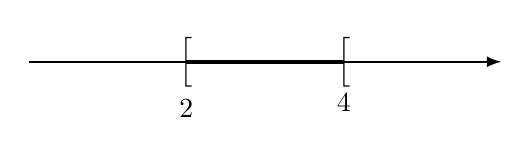
\begin{tikzpicture}[>=latex]
    \draw[thick,->] (0,0) --(6,0);
    \foreach \xp in {1,2,...,5}{\node[] at (\xp,0) {$\shortmid$};}
    \node[] at (2,0) {$\textbf{\Big[}$};
    \node[] at (4,0) {$\Big[$};
    \node[below=10pt] at (2,0) {$2$};
    \node[below=8pt] at (4,0) {$4$};
    \draw[ultra thick,-] (2,0) --(4,0);
\end{tikzpicture} \vspace{-2mm} \\ \hline 
$\left[ 3;+ \infty \right[$ &  & \begin{tikzpicture}[>=latex]
    \node[text=white] at (2,0) {$\textbf{\Big[}$};
    \node[text=white] at (4,0) {$\Big]$};
    \node[below=10pt,text=white] at (2,0) {$a$};
    \node[below=8pt,text=white] at (4,0) {$b$};
    \draw[ultra thick,-,draw=white] (2,0) --(4,0);
    \draw[thick,-,draw=white] (0,0) --(6,0);
\end{tikzpicture} \vspace{-2mm} \\ \hline 
 & $2<x<3$ et $4 \leq x$ & \begin{tikzpicture}[>=latex]
    \node[text=white] at (2,0) {$\textbf{\Big[}$};
    \node[text=white] at (4,0) {$\Big]$};
    \node[below=10pt,text=white] at (2,0) {$a$};
    \node[below=8pt,text=white] at (4,0) {$b$};
    \draw[ultra thick,-,draw=white] (2,0) --(4,0);
    \draw[thick,-,draw=white] (0,0) --(6,0);
\end{tikzpicture} \vspace{-2mm} \\ \hline 
 & & 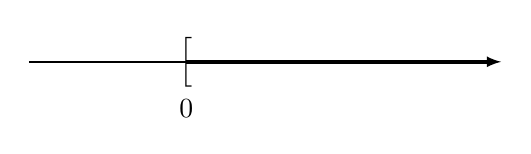
\begin{tikzpicture}[>=latex]
    \draw[thick,->] (0,0) --(6,0);
    \foreach \xp in {1,2,...,5}{\node[] at (\xp,0) {$\shortmid$};}
    \node[] at (2,0) {$\textbf{\Big[}$};
    \node[below=10pt] at (2,0) {$0$};
    \draw[ultra thick,-] (2,0) --(5.9,0);
\end{tikzpicture} \vspace{-2mm} \\ \hline
\end{tabularx}
\end{center}

\end{exercice}

\begin{exercice}
On considère l'intervalle $[-4;3]$. Citer un élément de cet intervalle qui soit:
\begin{enumerate}
\item Un entier naturel
\item Un entier mais pas naturel
\item Un décimal mais pas entier
\item Un rationnel mais pas décimal

\end{enumerate}

\end{exercice}

\begin{exercice}
En France, l'accès aux boîtes de nuit est réservée aux majeurs. Dans \textit{Le Macumba}, il faut avoir strictement plus de 32 ans pour entrer. Dans  \textit{La Playa}, il faut avoir au plus 40 ans.

\begin{enumerate}

\item Dans quel intervalle d'âge doit se situer une personne qui veut pouvoir rentrer dans les deux boîtes de nuit?

\item Dans quel ensemble doit se situer l'âge d'une personne qui veut pouvoir entrer dans l'une des deux boîtes de nuit?

\end{enumerate}

\end{exercice}

\begin{exercice}
Donner la valeur absolue des nombres suivants:
$$a) -5 \qquad b) 10 \qquad c) \enskip \frac {-2} {-3} \qquad d) \enskip 3-\frac 2 3 \times (6-4) \qquad e) - \sqrt {289}$$
\end{exercice}

\begin{exercice}
Donner la distance entre chaque pair de réels:
$$ a) -2 \text{ et} -12 \qquad b) -\pi \text{ et } 2 \pi \qquad c) \enskip \frac 5 3 \text{ et } \frac 7 6 \qquad d) -4 \text{ et } 6$$ 
\end{exercice}

\begin{exercice}
Résoudre les équations suivantes:
$$a) \abs x = 8 \qquad b) \abs x = -5 \qquad c) \abs {x-1} =  3 \qquad d) \abs{2x+1} = 4$$
\end{exercice}

\begin{exercice}
Déterminer et représenter les intervalles comprenant les réels $x$ tels que:
$$ a) \abs{x-2}\leq 1 \qquad b) \abs{x+1} \leq 2 \qquad \abs{x+3} \leq 3$$
\end{exercice}

\newpage

\titre{A projeter}

\vspace{3cm}

\begin{large}

\begin{exercice}

Représenter puis donner sous forme d'intervalle l'ensemble des nombres réels qui appartiennent à $]-1;1[$ et $[0;2]$.

\end{exercice}


\begin{exercice}

Compléter le tableau suivant: 

\begin{center}
\begin{tabularx}{\textwidth}{ 
  | >{\centering\arraybackslash}c 
  | >{\centering\arraybackslash}c
  | >{\centering\arraybackslash}X | }
\hline
Intervalle & Inégalité associée & Représentation\\ \hline 
$\hspace{1.5cm} \left] -4;-1 \right] \hspace{1.5cm}$ &  & \vspace{5mm} \begin{tikzpicture}[>=latex]
    \node[text=white] at (2,0) {$\textbf{\Big[}$};
    \node[text=white] at (4,0) {$\Big]$};
    \node[below=10pt,text=white] at (2,0) {$a$};
    \node[below=8pt,text=white] at (4,0) {$b$};
    \draw[ultra thick,-,draw=white] (2,0) --(4,0);
    \draw[thick,->,draw=white] (0,0) --(7,0);
\end{tikzpicture}  \\ \hline
 & $\hspace{1.5cm} -3 < x \leq 1 \hspace{1.5cm}$ & \vspace{5mm} \begin{tikzpicture}[>=latex]
    \node[text=white] at (2,0) {$\textbf{\Big[}$};
    \node[text=white] at (4,0) {$\Big]$};
    \node[below=10pt,text=white] at (2,0) {$a$};
    \node[below=8pt,text=white] at (4,0) {$b$};
    \draw[ultra thick,-,draw=white] (2,0) --(4,0);
\end{tikzpicture} \\ \hline
\end{tabularx}
\end{center}
\end{exercice}

\begin{exercice}
Représenter puis donner sous forme d'intervalle l'ensemble des nombres réels qui appartiennent à $[-1;3[$ et $]0;5]$.
\end{exercice}

\begin{exercice}
Compléter le tableau suivant:

\begin{center}
\begin{tabularx}{\textwidth}{ 
  | >{\centering\arraybackslash}c 
  | >{\centering\arraybackslash}X
  | >{\centering\arraybackslash}X | }
\hline
Intervalle & Inégalité associée & Représentation\\ \hline 
 & $2<x<3$ ou $4 \leq x$ & \begin{tikzpicture}[>=latex]
    \node[text=white] at (2,0) {$\textbf{\Big[}$};
    \node[text=white] at (4,0) {$\Big]$};
    \node[below=10pt,text=white] at (2,0) {$a$};
    \node[below=8pt,text=white] at (4,0) {$b$};
    \draw[ultra thick,-,draw=white] (2,0) --(4,0);
    \draw[thick,-,draw=white] (0,0) --(6,0);
\end{tikzpicture} \vspace{-2mm} \\ \hline 
 & & 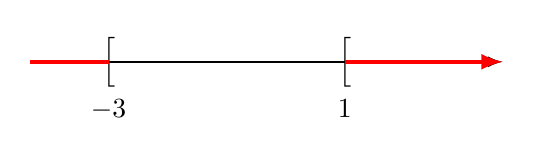
\begin{tikzpicture}[>=latex]
    \draw[thick,->] (0,0) --(6,0);
    \foreach \xp in {1,2,...,5}{\node[] at (\xp,0) {$\shortmid$};}
    \node[] at (4,0) {$\textbf{\Big[}$};
    \node[] at (1,0) {$\textbf{\Big[}$};
    \node[below=10pt] at (1,0) {$-3$};
    \node[below=10pt] at (4,0) {$1$};
    \draw[ultra thick,->,draw=red] (4,0) --(6,0);
    \draw[ultra thick,-,draw=red] (0,0) --(1,0);

\end{tikzpicture} \vspace{-2mm} \\ \hline
\end{tabularx}
\end{center}

\end{exercice}

\end{large}

\end{document}
